\documentclass[12pt,fleqn]{article}
\usepackage{
  amsmath,
  amssymb,
  booktabs,
  geometry,
  graphicx,
  microtype,
  parskip,
  caption,
}
\usepackage[shortlabels]{enumitem}

\geometry{margin=3cm}

% equation line spacing
\setlength{\jot}{0.5cm}

% meta data
\newcommand{\chapter}{6.2}
\newcommand{\authorname}{Amo DelBello}
\newcommand{\classdescription}{MATH 1350-D2}
\newcommand{\classname}{Introduction to Statistics, Fall 2022}
\newcommand{\assignment}{\chapter\ Book Assignment}

\newcommand{\problem}[1]{\vspace{5ex}\section*{\chapter-#1}}
\newcommand{\thead}[1]{\textnormal{\textbf{#1}}}
\newcommand{\tvspace}{\vspace{.25cm}}

\title{\classdescription\ \\ \classname\ \\ $\ $ \\ \assignment}
\author{\authorname}
\date{\today}


\begin{document}

\maketitle

(I used StatCrunch to calculate the answers for all of the problems in the section.)

\problem{5}
0.8849


\problem{6}
0.7257


\problem{7}
0.9053


\problem{8}
0.1571


\problem{21}
\begin{enumerate}[label=\alph*.]
\item $72.11\%$ of women meet the height requirement. $27.89\%$ of women do not meet the requirement, which could be considered as ``many.''

\item The new height requirements for women would be 58.2 in. to 69.2 in.

\begin{figure}[ht]
  \centering
  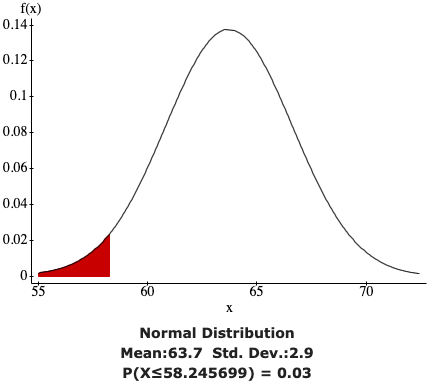
\includegraphics[width=8cm]{assets/21-navy-left.png}
\end{figure}
\begin{figure}[ht]
  \centering
  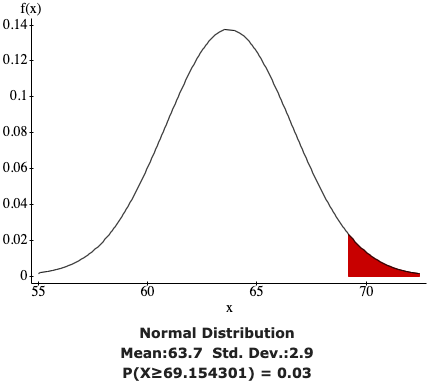
\includegraphics[width=8cm]{assets/21-navy-right.png}
\end{figure}

\end{enumerate}


\problem{26}
\begin{enumerate}[label=\alph*.]
\item The minimum table clearance required to satisfy the requirement of fitting 95\% of men is 19.43 in. I'm not sure why the 95th percentile for women is ignored in this case. Perhaps it is because the minimum clearance for men happens to be the approximate mean for women, so most women would be accommodated. Additionally, maybe these work stations are primarily used by men, so it's less important to satisfy a minority of users at the expense of the majority.

\item The table fits 4.01\% of men and 0.0002\% of women. It appears to be made to fit almost no one.
\end{enumerate}


\problem{30}
\begin{enumerate}[label=\alph*.]
\item $1 - 0.0001938 = 0.9998062 = 99.98\%$ of people would be considered to have a fever. This percentage suggests that a cutoff of $100.4^\circ F$ is appropriate.

\item $96.93^\circ F$ would be the minimum temperature that only 2.0\% of people would exceed.
\end{enumerate}

\end{document}
%%% Local Variables:
%%% mode: latex
%%% TeX-master: t
%%% End:
